\chapter{La historia del dinero}

\section{Introducción}

El concepto de dinero ha sido fundamental en el desarrollo de las civilizaciones humanas. Desde los sistemas de trueque hasta las monedas digitales, el dinero ha evolucionado enormemente a lo largo de la historia, facilitando el comercio y la interacción entre diferentes culturas. Este capítulo ofrece un recorrido por la historia del dinero, desde sus primeras formas hasta los sistemas financieros modernos.

\section{El trueque y las primeras formas de dinero}

Antes de la invención del dinero tal como lo conocemos hoy, las civilizaciones utilizaban el trueque, un sistema en el que los bienes y servicios se intercambiaban directamente. Sin embargo, este sistema tenía limitaciones importantes. Por ejemplo, para que el trueque funcionara, ambas partes debían tener algo que la otra quisiera, lo que se conoce como la \textit{doble coincidencia de deseos}.

Para superar estas limitaciones, las civilizaciones comenzaron a utilizar ciertos objetos como medios de intercambio. Algunos ejemplos tempranos de dinero incluyen el uso de conchas, piedras, ganado, y otros bienes que tenían valor intrínseco o eran escasos.

\section{El surgimiento de las monedas}

Una de las primeras formas de dinero que no estaba vinculada a un bien específico fue la moneda de metal. En el siglo VII a.C., los lidios, una civilización en lo que ahora es Turquía, fueron los primeros en acuñar monedas de una aleación de oro y plata llamada \textit{electrum}. Estas monedas estandarizadas permitieron transacciones más eficientes, ya que eran fáciles de transportar y su valor era claro para todas las partes involucradas.

El uso de monedas rápidamente se extendió por otras civilizaciones, como los griegos, los romanos y los chinos, quienes también comenzaron a acuñar sus propias monedas. En cada sociedad, el diseño y valor de las monedas variaba, pero su función como medio de intercambio y reserva de valor era universal.

\begin{imagen}[h!]
	\centering
	\includegraphics[width=\textwidth]{./media/coin.png}
	\caption{Antiguas monedas acuñadas.}
\end{imagen}

\section{El papel moneda y la bancarización}

Con el tiempo, las monedas de metal se volvieron difíciles de manejar en grandes cantidades, especialmente para las transacciones comerciales. Esto llevó al surgimiento del papel moneda. El uso del papel moneda se originó en China durante la dinastía Tang (618-907 d.C.), donde se utilizaba como recibo de depósitos de metales preciosos.

En Europa, el papel moneda fue introducido más tarde, principalmente por los bancos que emitían notas bancarias respaldadas por reservas de oro y plata. Estas notas podían ser intercambiadas por el valor equivalente en metales preciosos, lo que facilitó el comercio y el desarrollo de los mercados financieros.

\subsection{Cifras clave de la historia del dinero}

En el cuadro~\ref{moneyhistory}, se observan algunos eventos históricos clave en la evolución del dinero y sus correspondientes fechas.

\begin{table}[!ht]
\sf\footnotesize\setlength\tabcolsep{4pt}
\centering
\begin{tabular}{l | S[table-format=4.0]}
\toprule
\textbf{Evento} & \textbf{Año} \\
\midrule
Primera acuñación de monedas en Lidia & 700 \\
\midrule
Introducción del papel moneda en China & 618 \\
\midrule
Primera casa de moneda en Roma & 289 \\
\midrule
Establecimiento del patrón oro en el Reino Unido & 1821 \\
\midrule
Primera emisión de dólares en EEUU & 1792 \\
\midrule
Abolición del patrón oro & 1971 \\
\bottomrule
\end{tabular}
\caption{Eventos importantes en la historia del dinero.}\label{moneyhistory}
\end{table}

\section{La era digital y el futuro del dinero}

En la actualidad, el dinero ha dado un giro hacia lo digital. Las transacciones electrónicas han superado al uso de efectivo en muchas partes del mundo. Con la invención de las criptomonedas, como Bitcoin, estamos viendo una transformación aún más radical en cómo las personas perciben y utilizan el dinero.

Las criptomonedas son un tipo de dinero digital que utiliza la tecnología de \textit{blockchain} para garantizar transacciones seguras sin la necesidad de intermediarios como bancos o gobiernos. Aunque su uso todavía no está generalizado, las criptomonedas han generado un debate significativo sobre el futuro del dinero y los sistemas financieros.

\begin{figure}[!ht]
\begin{mdframed}[backgroundcolor=gray!5,linewidth=0.5pt]
\centering
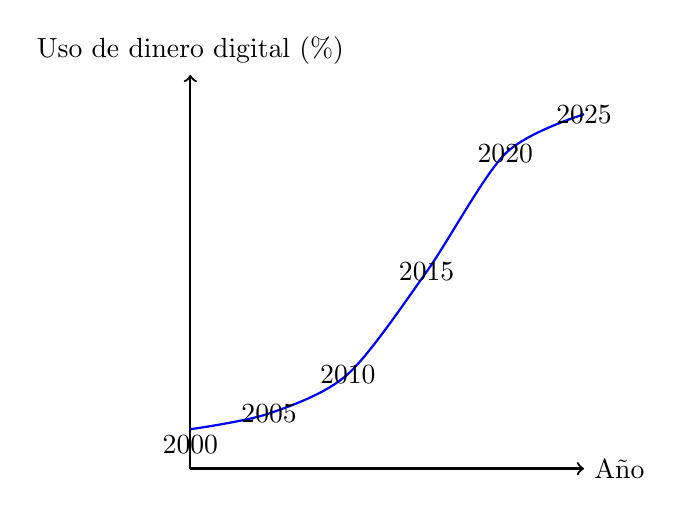
\begin{tikzpicture}
% Axes
\draw[thick,->] (0,0) -- (5,0) node[right] {Año};
\draw[thick,->] (0,0) -- (0,5) node[above] {Uso de dinero digital (\%)};

% Data points
\draw[thick, color=blue] plot[smooth] coordinates {(0,0.5) (1,0.7) (2,1.2) (3,2.5) (4,4) (5,4.5)};

% Labels
\node at (0,0.3) {2000};
\node at (1,0.7) {2005};
\node at (2,1.2) {2010};
\node at (3,2.5) {2015};
\node at (4,4) {2020};
\node at (5,4.5) {2025};
\end{tikzpicture}
\end{mdframed}
\caption{Crecimiento del uso de dinero digital.}\label{monedas}
\end{figure}

\section{Conclusiones}

La evolución del dinero refleja no solo cambios en la tecnología y la economía, sino también en la sociedad y la cultura. Desde los primeros sistemas de trueque hasta las monedas digitales descentralizadas, el dinero ha sido un motor clave para el progreso humano. En el futuro, el dinero continuará evolucionando a medida que las nuevas tecnologías y modelos económicos surjan, cambiando la manera en que interactuamos con la economía global.

